\documentclass[a4paper,12pt]{article}
\usepackage[utf8]{inputenc}
\usepackage[T1]{fontenc}
\usepackage[toc,page]{appendix} 
\usepackage[frenchb]{babel}
\usepackage{xspace}
\usepackage[round,authoryear]{natbib}
\usepackage{graphicx} %
\usepackage[table,dvipsnames]{xcolor} %Couleurs dans les tableaux (cellules, colonnes, etc.)
\usepackage{url} %Formatage hyperlinks
\usepackage{float} 
\usepackage{wrapfig} %Placement fin des figures dans les pages
\usepackage{booktabs} % 
\usepackage{caption}
\usepackage{subcaption}
\usepackage{glossaries}
\usepackage{acronym}
\usepackage{amssymb}
\usepackage{amsmath}
\usepackage{mathtools}
\usepackage[pagebackref=true]{hyperref}
\usepackage[toc,page]{appendix}
\usepackage{pdflscape}
\usepackage{multirow}
\usepackage{rotating}
\usepackage{color,colortbl}
\usepackage[final]{pdfpages} % pour la couverture
\usepackage[only]{excludeonly}
\usepackage{lmodern}
\usepackage{hhline}
\usepackage{relsize}
\title{Résultats}



\graphicspath{./images/}


\begin{document}
\maketitle

\section{Application aux rues de Paris}
\paragraph{Sources géohistoriques traitées}
Dans cette section, nous appliquons l'approche de construction de graphe géohistoriques aux réseaux des rues de Paris extrait des différents atlas parisiens traités dans les chapitres précédents. Les quatre atlas dont les rues ont été vectorisés sont les suivants~:
\begin{itemize}
\item l'atlas de Verniquet, dont le temps valide est le sous-ensemble flou (1783, 1785, 1791, 1799),
\item l'atlas par îlots de Vasserot, entièrement vectorisé par \cite{ALPAGE}, dont nous avons fixé le temps valide (1808, 1810, 1836, 1854),
\item l'atlas de Jacoubet, de temps valide (1825, 1827, 1836, 1837),
\item l'atlas municipal de Paris de l'année 1888, de temps valide (1887, 1888, 1889),
\end{itemize}
Le temps valide désigne la période pendant laquelle les observations des entités du monde réel sont effectuées puis transcrites dans l'atlas. Par exemple, nous considérons que l'atlas de Verniquet décrit des entités du monde réel ayant existé entre 1783 et 1799. La certitude de cette hypothèse n'est pas toujours totale, ce qui est exprimé par l'utilisation des sous-ensembles temporels flous. Ainsi, nous sommes sûrs que l'atlas de Verniquet ait pu permettre l'observation d'entités du monde réel entre 1785 et 1791 c'est à dire la période de levé topographique et de dessin de l'atlas. Avant 1785 et après 1791, il est de moins en moins certain que des relevés ou des corrections aient été effectuées.
\\
La figure~\ref{figure:temps_valides_tous_plans} illustre la localisation temporelle de ces différents atlas. On peut remarquer que le temps valide de l'atlas de Jacoubet est totalement inclus dans celui de l'atlas de Vasserot. Cela signifie que la méthode de construction du graphe considérera comme possible l'existence de relations de filiations allant de Vasserot à Jacoubet ou de Jacoubet vers Vasserot.
\\
Nous n'avons pas l'information détaillée des temps valide pour chaque observations vectorisée des rues de Paris. Bien que ces informations puissent être extraites de sources telles que les dictionnaires de rues (voir \citep{Lazare1844, Lazare1855}), leur saisie dépasse de la cadre de cette thèse. Pour cette raison, \textbf{nous avons considéré que les observations des rues de Paris ont le même temps valide que leur source géohistorique}.

\begin{figure}
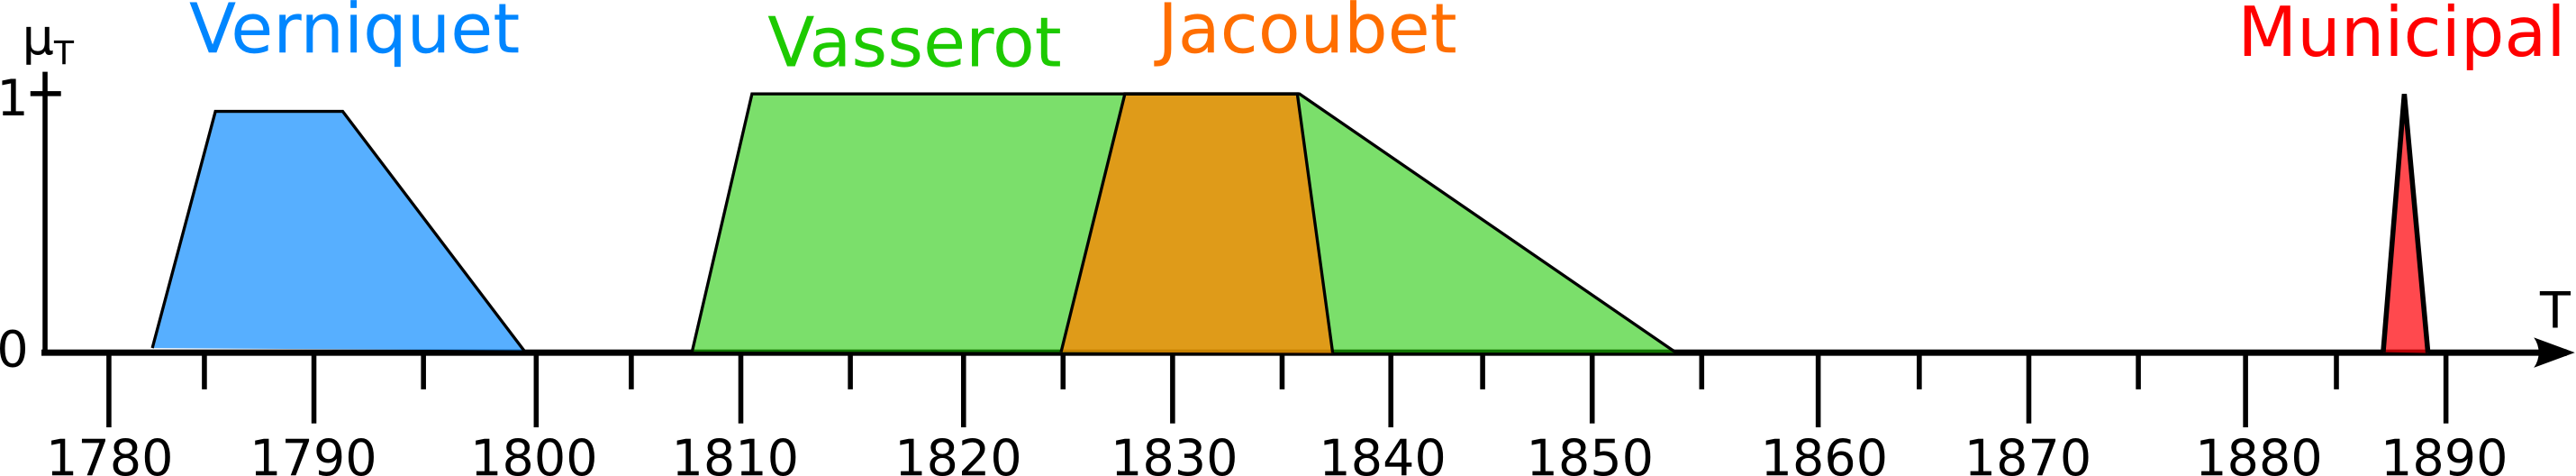
\includegraphics[width=1\textwidth]{./images/ftime_all_rappel.png}
\end{figure}

\paragraph{Représentation des réseaux viaires dans la base de données spatiale et temporelle}
Les réseaux de rues vectorisés et présentés en fin du chapitre 3 sont des graphes planaires topologiquement justes. Chaque réseau de rue vectorisé a été stocké comme un \emph{snapshot} vecteur de notre base de données géohistorique. Les observations géohistoriques de ces \emph{snapshots} sont des tronçons de rues, et non des rues au sens commun du terme (c'est-à dire un ensemble contigu de tronçons portant le même nom). Dans la base de données spatiale et temporelle, ces observations sont modélisées sous la forme de \emph{feature} linéaires\footnote{\emph{Linestrings} du schéma simple feature access}. La nature de ces observations est importante à garder en tête, en particulier pour l'étape de typage des filiations. En effet, ce ne seront alors pas les relations de filiations entre rues qui seront identifiées, mais les relations de filiation entre tronçons. Les transformations de l'espace qui en résultent sont donc également entre tronçons. La figure~\ref{fig:troncons} illustre ainsi le découpage du réseau viaire en tronçons de rues représentés sous la forme de \emph{features} linéaires. Cette figure présente tout d'abord le schéma de donnée aligné des tronçons de rue issus des différents \emph{snapshots}que nous utilisons pour tester notre méthode (\ref{fig:schema_aligne_tronçons}), puis illustre le découpage du réseau en tronçons pour les \emph{snapshots} des tronçons de Verniquet, Vasserot et Jacoubet (\ref{fig:extract_tronc}). Enfin, un extrait du snapshot des tronçons de l'atlas de Verniquet est présenté en figure \ref{fig:extract_snap}. Les champs \emph{vtime} (temps valide) et \emph{the\_geom} (géométrie) sont figurés sous forme textuelle pour la lecture. Rajoutons que l'alignement des schémas des réseaux viaires a été réalisé manuellement au moment du versement des réseaux dans la base de données.
\begin{figure}[H]
        \centering
        \begin{subfigure}[b]{0.3\textwidth}
                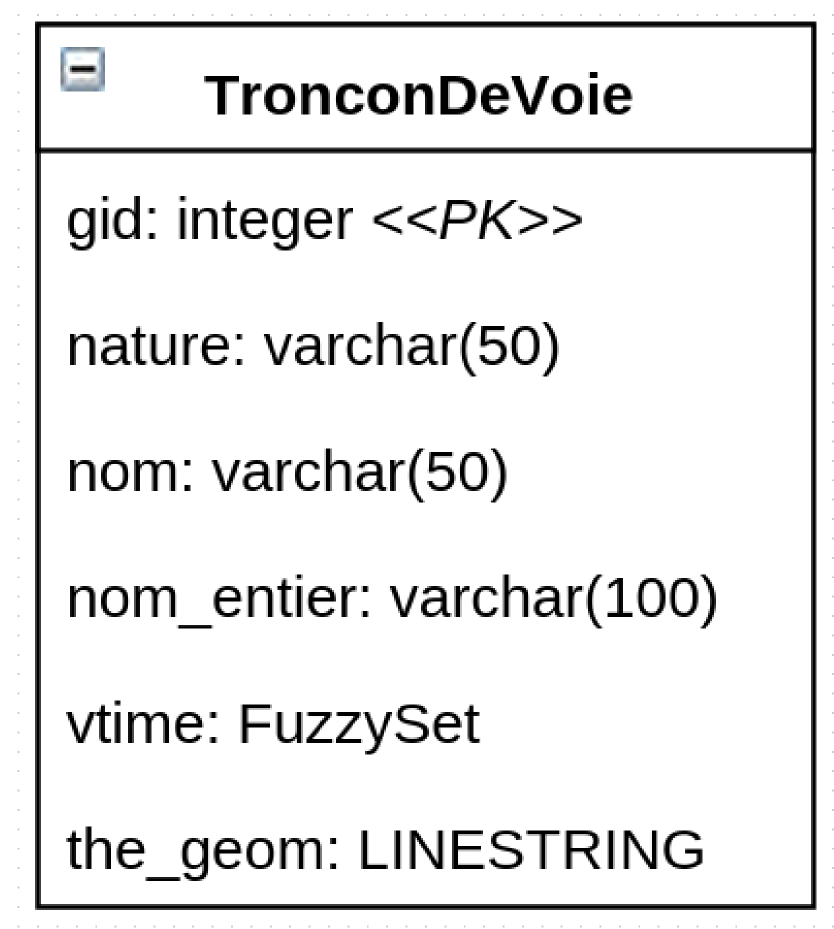
\includegraphics[width=\textwidth]{./images/schema_bd_tronc.png}
				\caption{Schéma commun des tronçons des réseaux viaires de Paris.}
                \label{fig:schema_aligne_tronçon}
        \end{subfigure}%v
        \\
        \begin{subfigure}[b]{1\textwidth}
                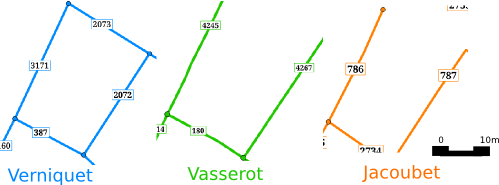
\includegraphics[width=\textwidth]{./images/extract_tronc_3src.png}
				\caption{Extraits des réseaux viaires stockés.}
                \label{fig:extract_tronc}
        \end{subfigure}
        \\
        \begin{subfigure}[b]{1\textwidth}
                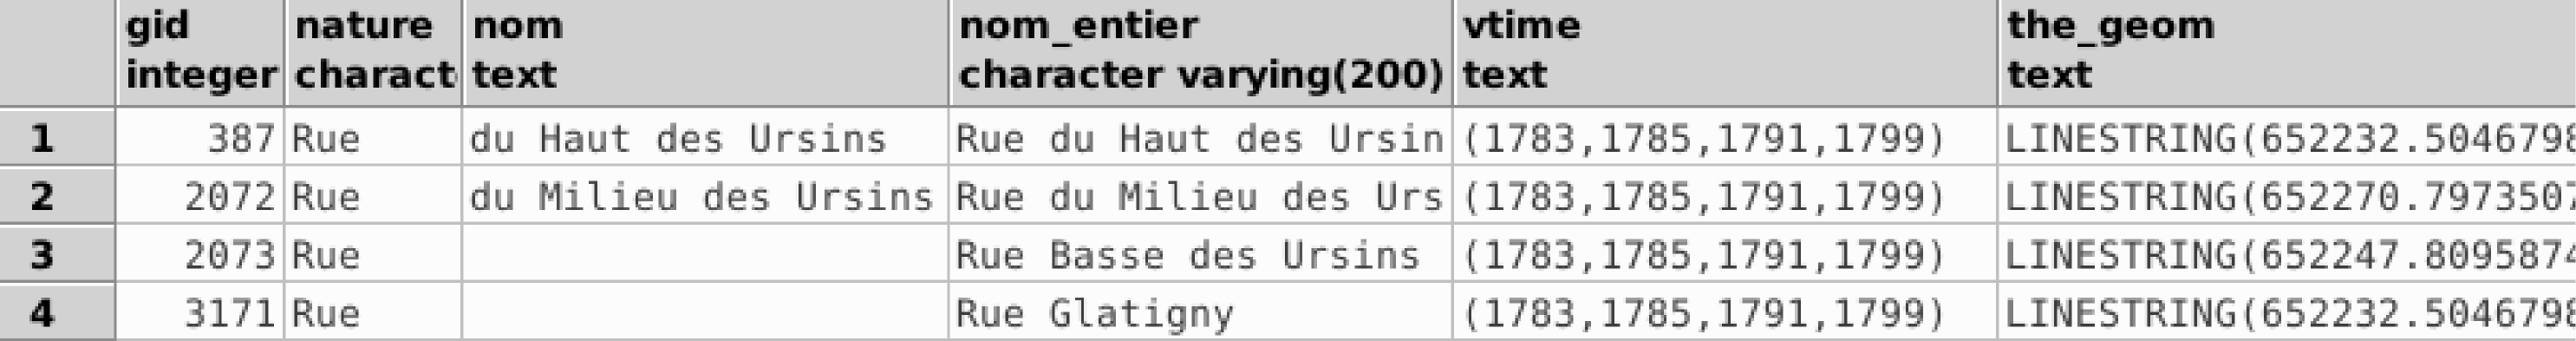
\includegraphics[width=\textwidth]{./images/extract_bd_vern.png}
                \caption{Extrait de la base de données spatiale et temporelle.}
                \label{fig:extract_snap}
        \end{subfigure}
        \label{fig:troncons}
	    \caption{Modélisation des réseaux viaires de Paris dans la base de données spatiale et temporelle}
\end{figure}

\paragraph{Décalages planimétriques}
En raison des erreurs de levé topographique et des erreurs résiduelles dues au géoréférencement des planches des atlas, les réseaux de rue présentent des décalages. L'amplitude de ces erreurs peut varier fortement selon les zones de l'espace parisien, allant de quelques mètres dans le centre parisien de la rive droite à plus de 10 mètres pour les impasses, passages et cul-de sacs souvent présents dans les îlots anciens. Ces décalages peuvent être également dû aux élargissements des voies. En effet, puisque seuls les axes centraux des rues ont été vectorisés, un élargissement à droite ou à gauche d'une rue décale son axe. Deux situations sont présentées en figure \ref{fig:extrait_decalage}, avec tous les réseaux superposés. À gauche, la partie nord de l'île Saint-Louis, presque inchangée, présente des décalages faibles. À l'inverse, la vignette de droite montre les décalages de rues et passages à l'intérieur d'un îlot, où les décalages planimétriques approchent 10 mètres. L'erreur est particulièrement importante pour les tronçons issus de l'atlas de Jacoubet (en orange).

\begin{figure}
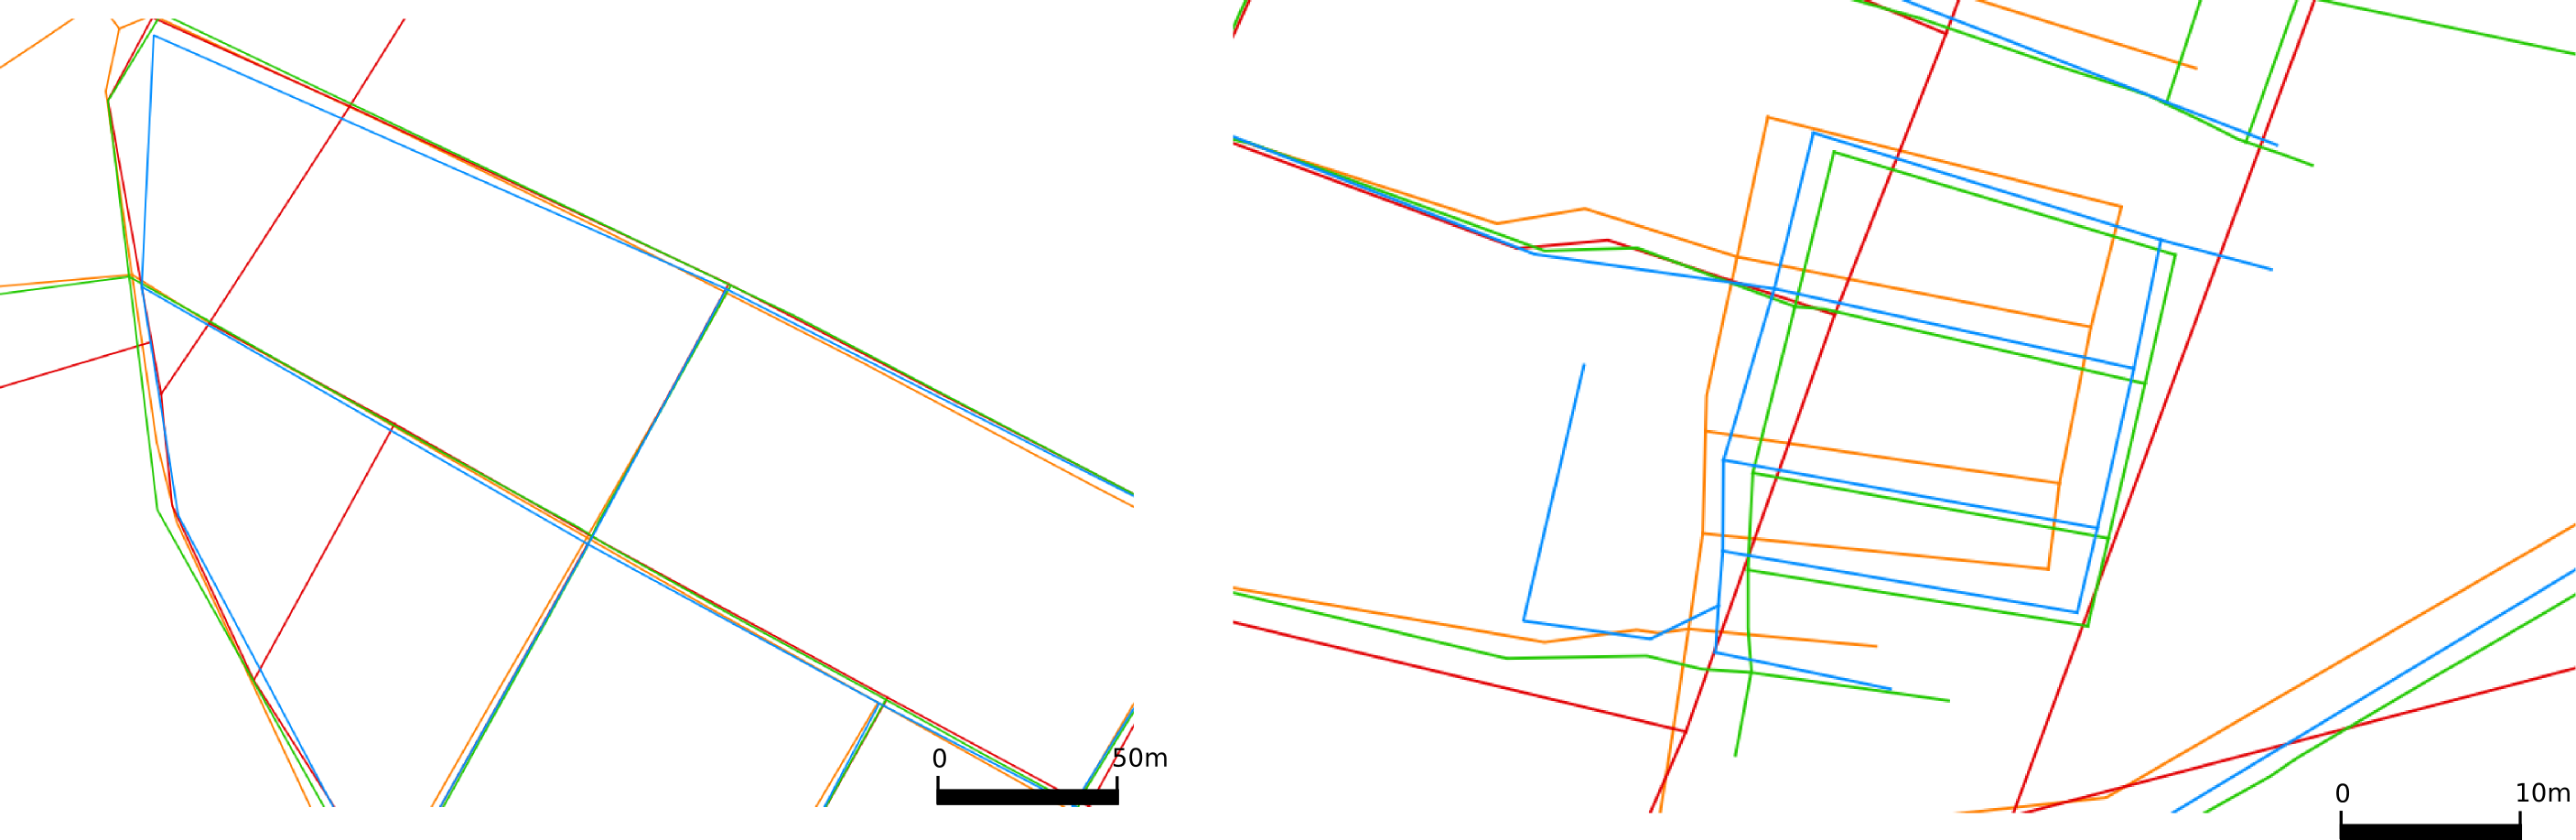
\includegraphics[width=1\textwidth]{./images/ex_decalages.png}
\caption{Illustration des décalages planimétriques entre réseaux viaires sur l'île saint Louis et l'îlot de la trinité.}
\label{fig:extrait_decalage}
\end{figure}
\subsection{Mesures utilisées}


\subsection{Première Zone~: ancien îlot de la Trinité}
\paragraph{Données utilisées}
nombre de tronçons.
\paragraph{Paramètres utilisés pour la phase de découverte des relations}
Il y a deux catégories de paramètres à définir : ceux qui concernent les critères d'appariement (il y en a au minimum un par critère) et ceux qui concernent le recuit simulé.
Dans la première catégorie, il y a~:
\begin{itemize}
\item Le seuil de la distance de Fréchet,
\item Le seuil de sauts temporels,
\item le voisinage ST
\end{itemize}
Le seuil d'antériorité temporelle n'a pas besoin d'être défini puisque le critère est déjà centré autour de 0.5.
\\
Dans la seconde catégorie, il y a~:
\begin{itemize}
\item la température initiale
\item le ratio de décroissance de température
\item le nombre d'itérations max
\item le critère d'arrêt (stagnation).
\end{itemize}

\paragraph{paramètres utilisés pour la phase de typage}
Il faut définir les différentes fonctions de croyance.

\paragraph{Résultats et commentaires des résultats}
Try 1 : Stop a 20k iterations
temps : 12.787 (i=6817), 13.07 (i=5798), 12.026 (6471), 11.91 (7548) , 15.069(7966)


Vrai essai (celui des figures ) : 50k iterations, 60s, energy du meilleur graphe = -151.894515 avec 25 hyperarcs. 0.14 de variation moyenne de l'énergie. 
\\
Commentaires : le matching est bon, on remarque le sur-appariement entre vasserot et jacoubet. C'est le cas où il n'y a pas de pénalité pour les NM
\begin{figure}
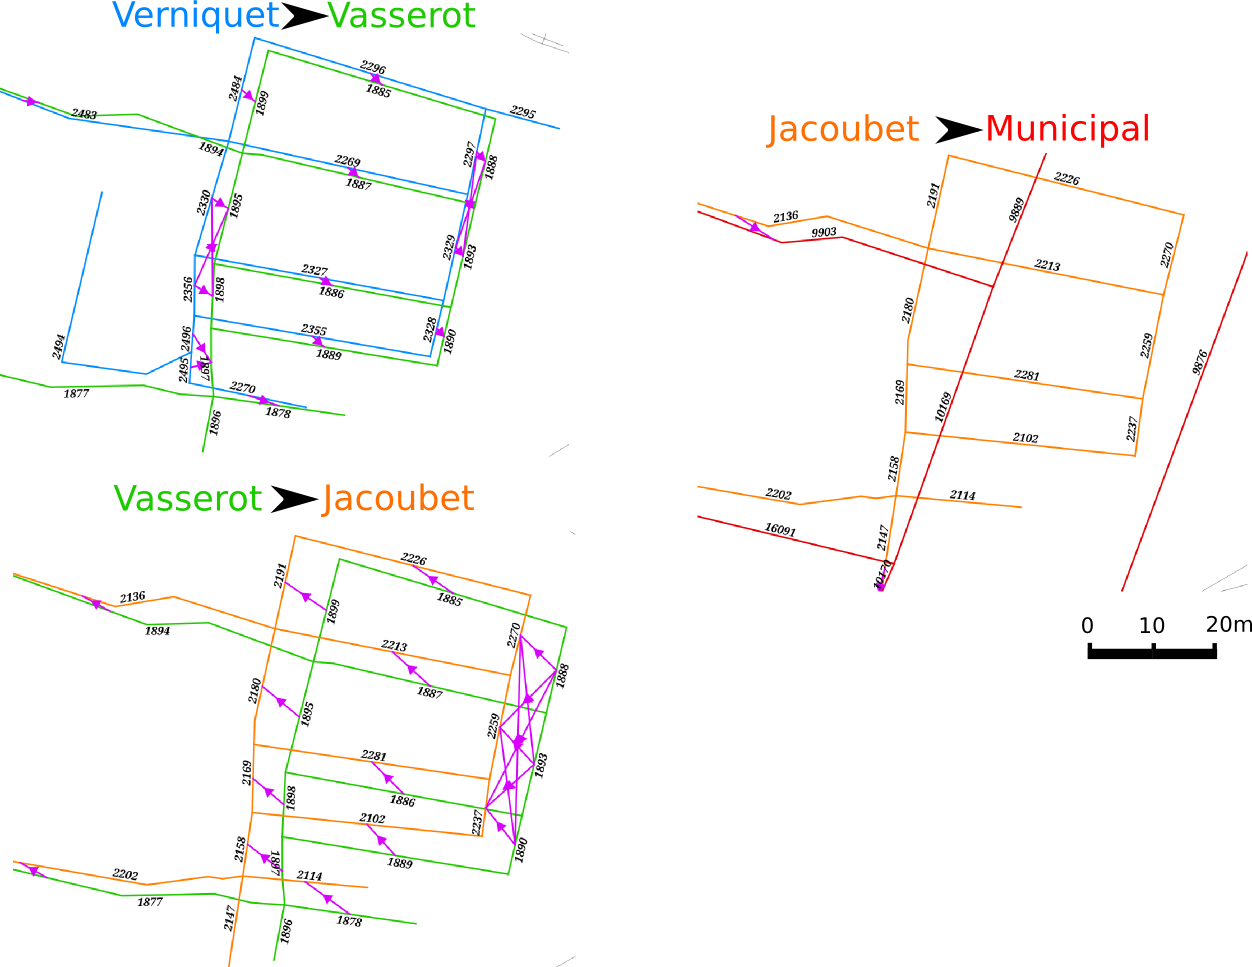
\includegraphics[angle = 90, width=1\textwidth]{./images/illus_graphs/graphe_troncons_greneta.png}
\end{figure}

Le cas où il y  a une pénalité sur les NMS est dans la figure ci-dessous :
\begin{figure}
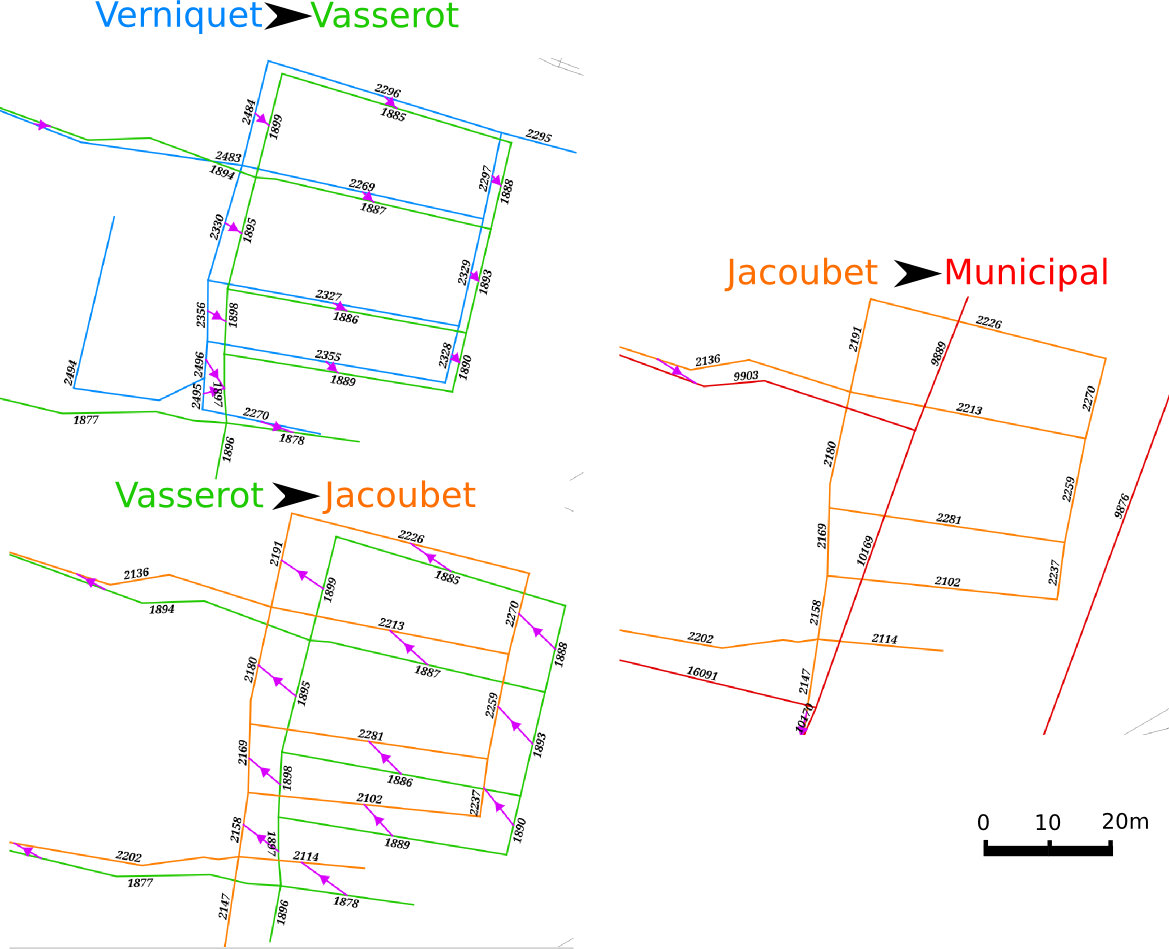
\includegraphics[angle = 90, width=1\textwidth]{./images/illus_graphs/graphe_troncons_greneta_nmpenalty.png}
\end{figure}


\paragraph{comparaison avec la vérité terrain avec NMS}
\begin{table}
\caption{Qualité de l'appariement sur le quartier Greneta}
\begin{tabular}{c|c|c|c|c|}
Méthode & Snapshots & Rappel & Précision & Fmesure \\ \hline
M\&D & Verniquet $\to$ Vasserot &  0.93 & 2 & 0.963 \\ \hline
- & Vasserot $\to$ Jacoubet &  1 & 1 & 1 \\ \hline
- & Jacoubet $\to$ Poubelle &  1 & 0.67 & 0.8 \\ \hline
\hline
Notre méthode & Verniquet $\to$ Vasserot &  1 & 0.77 & 0.875 \\ \hline
- & Vasserot $\to$ Jacoubet &  0.93 & 0.63 & 0.76 \\ \hline
- & Jacoubet $\to$ Poubelle &  1 & 1 & 1 \\ \hline
\hline
Après tagging (min 10m) & Verniquet $\to$ Vasserot &  1 & 0.93 & 0.965 \\ \hline
- & Vasserot $\to$ Jacoubet &  0.93 & 0.875 & 0.90 \\ \hline
- & Jacoubet $\to$ Poubelle &  1 & 1 & 1 \\ \hline
\hline
Avec Pénalité (+0.1 de croyance) & Verniquet $\to$ Vasserot &  1 & 1 & 1 \\ \hline
- & Vasserot $\to$ Jacoubet &  0.93 & 1 & 0.96 \\ \hline
- & Jacoubet $\to$ Poubelle &  1 & 1 & 1 \\ \hline

\end{tabular}
\end{table}

\paragraph{Résultat de l'étape de typage et commentaires sur la résolution des conflits}



\subsection{Seconde Zone~: Quartier des Arts et Métiers}
Ici c'est l'occasion de montrer les pb de convergence de l'algo.
\paragraph{Comparaison avec la vérité terrain}
\begin{table}
\caption{Qualité de l'appariement sur le quartier Saint Martin}
\begin{tabular}{c|c|c|c|c|}
Méthode & Snapshots & Rappel & Précision & Fmesure \\ \hline
M\&D & Verniquet $\to$ Vasserot &  0.836 & 0.98 & 0.90 \\ \hline
- & Vasserot $\to$ Jacoubet &  0.75 & 0.86 & 0.8 \\ \hline
- & Jacoubet $\to$ Municipal &  0.30 & 0.90 & 0.45 \\ \hline
\hline
Notre méthode & Verniquet $\to$ Vasserot &  0.95 & 0.90 & 0.93 \\ \hline
- & Vasserot $\to$ Jacoubet &  0,76 & 0.71 & 0.736 \\ \hline
- & Jacoubet $\to$ Municipal & 0.52 & 0.74 & 0.61 \\ \hline
\hline
Uniquement entre 3 et 4 (100k iter, t0 = 2, dec = 0.9999, frechet = 25)& Jacoubet $\to$ Municipal &  0.64 & 0.78 & 0.70 \\ \hline
\hline
Après tagging (15m) & Verniquet $\to$ Vasserot &  0.95 & 0.98 & 0.96 \\ \hline
- & Vasserot $\to$ Jacoubet &  0,78 & 0.78 & 0.78 \\ \hline
- & Jacoubet $\to$ Municipal & 0.52 & 0.94 & 0.67 \\ \hline
\hline

\end{tabular}
\end{table}


\paragraph{Convergence de l'algorithme d'appariement}
Problème induit par les NMS ~: pourquoi ça se passe, comment serait-il possible de le régler? Noter que çe problème là arrive égakelement dans les cas de 1-N et N-1 lorsque les tronçons de la première base sont très petits et ceux de la seconde très grands (ou vice versa). Pour régler le problème,une possibilité est d'opter pour un mode bcp plus optimiste dans lequel Frechet va placer dans l'ignorance plutôt que dans l'hypothèse "non app". En faisant ça, la probalitié pignistique d'un hyperarc est toujours supérieur à 0.5. Cela signifie que la mort et naissance est le pire des cas , ou, autrement dit, une observation disparait (resp apparait) lorsqu'aucune autre observation n'est disponible pour être son étant suivant (resp. précédent).



\subsection{Cartographies des transformations de Paris (bonus?)}

\subsection{Discussion}
\paragraph{Approche pessimiste versus optimiste}
\paragraph{Découpage en 2 étapes utile?}
\paragraph{Intégrer le recalage}
\paragraph{Prise en compte de la topologie}
\paragraph{Améliorer la convergence de la méthode}
\paragraph{Paramétrisation de la phase de typage (apprentissage?)}


Paramètres utilisés~:
\begin{itemize}
\item 30 0000 iterations
\item Température initiale de 1
\item Seuil de Fréchet de 10m
\end{itemize}



\subsection{Résultats et discussion}
Nous présentons ici les résultats obtenus par l'algorithme de découverte des relations de filiation sur quatre quartiers différents de Paris et sur les réseaux viaires issus des atlas de Verniquet, Vasserot, Jacoubet et de l'atlas municipal. 


\subsubsection{Greneta}

\begin{figure}
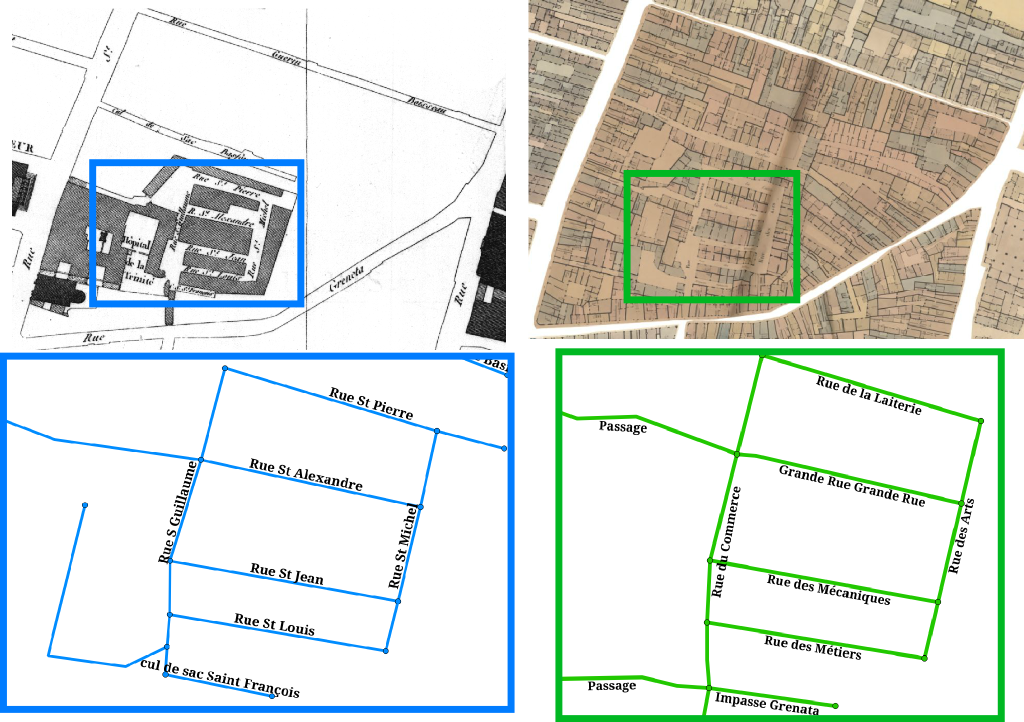
\includegraphics[width=1\textwidth]{./images/greneta_A.png}
\caption{Greneta A}
\end{figure}





\begin{figure}
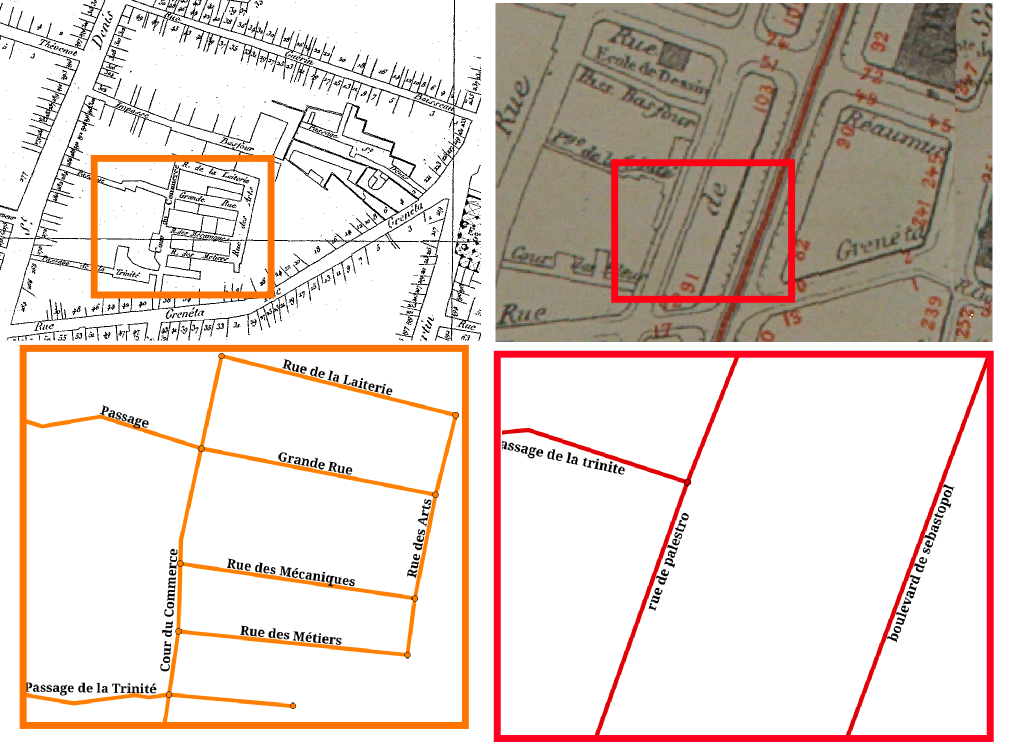
\includegraphics[width=1\textwidth]{./images/greneta_B.png}
\caption{Greneta B}
\end{figure}

\begin{figure}
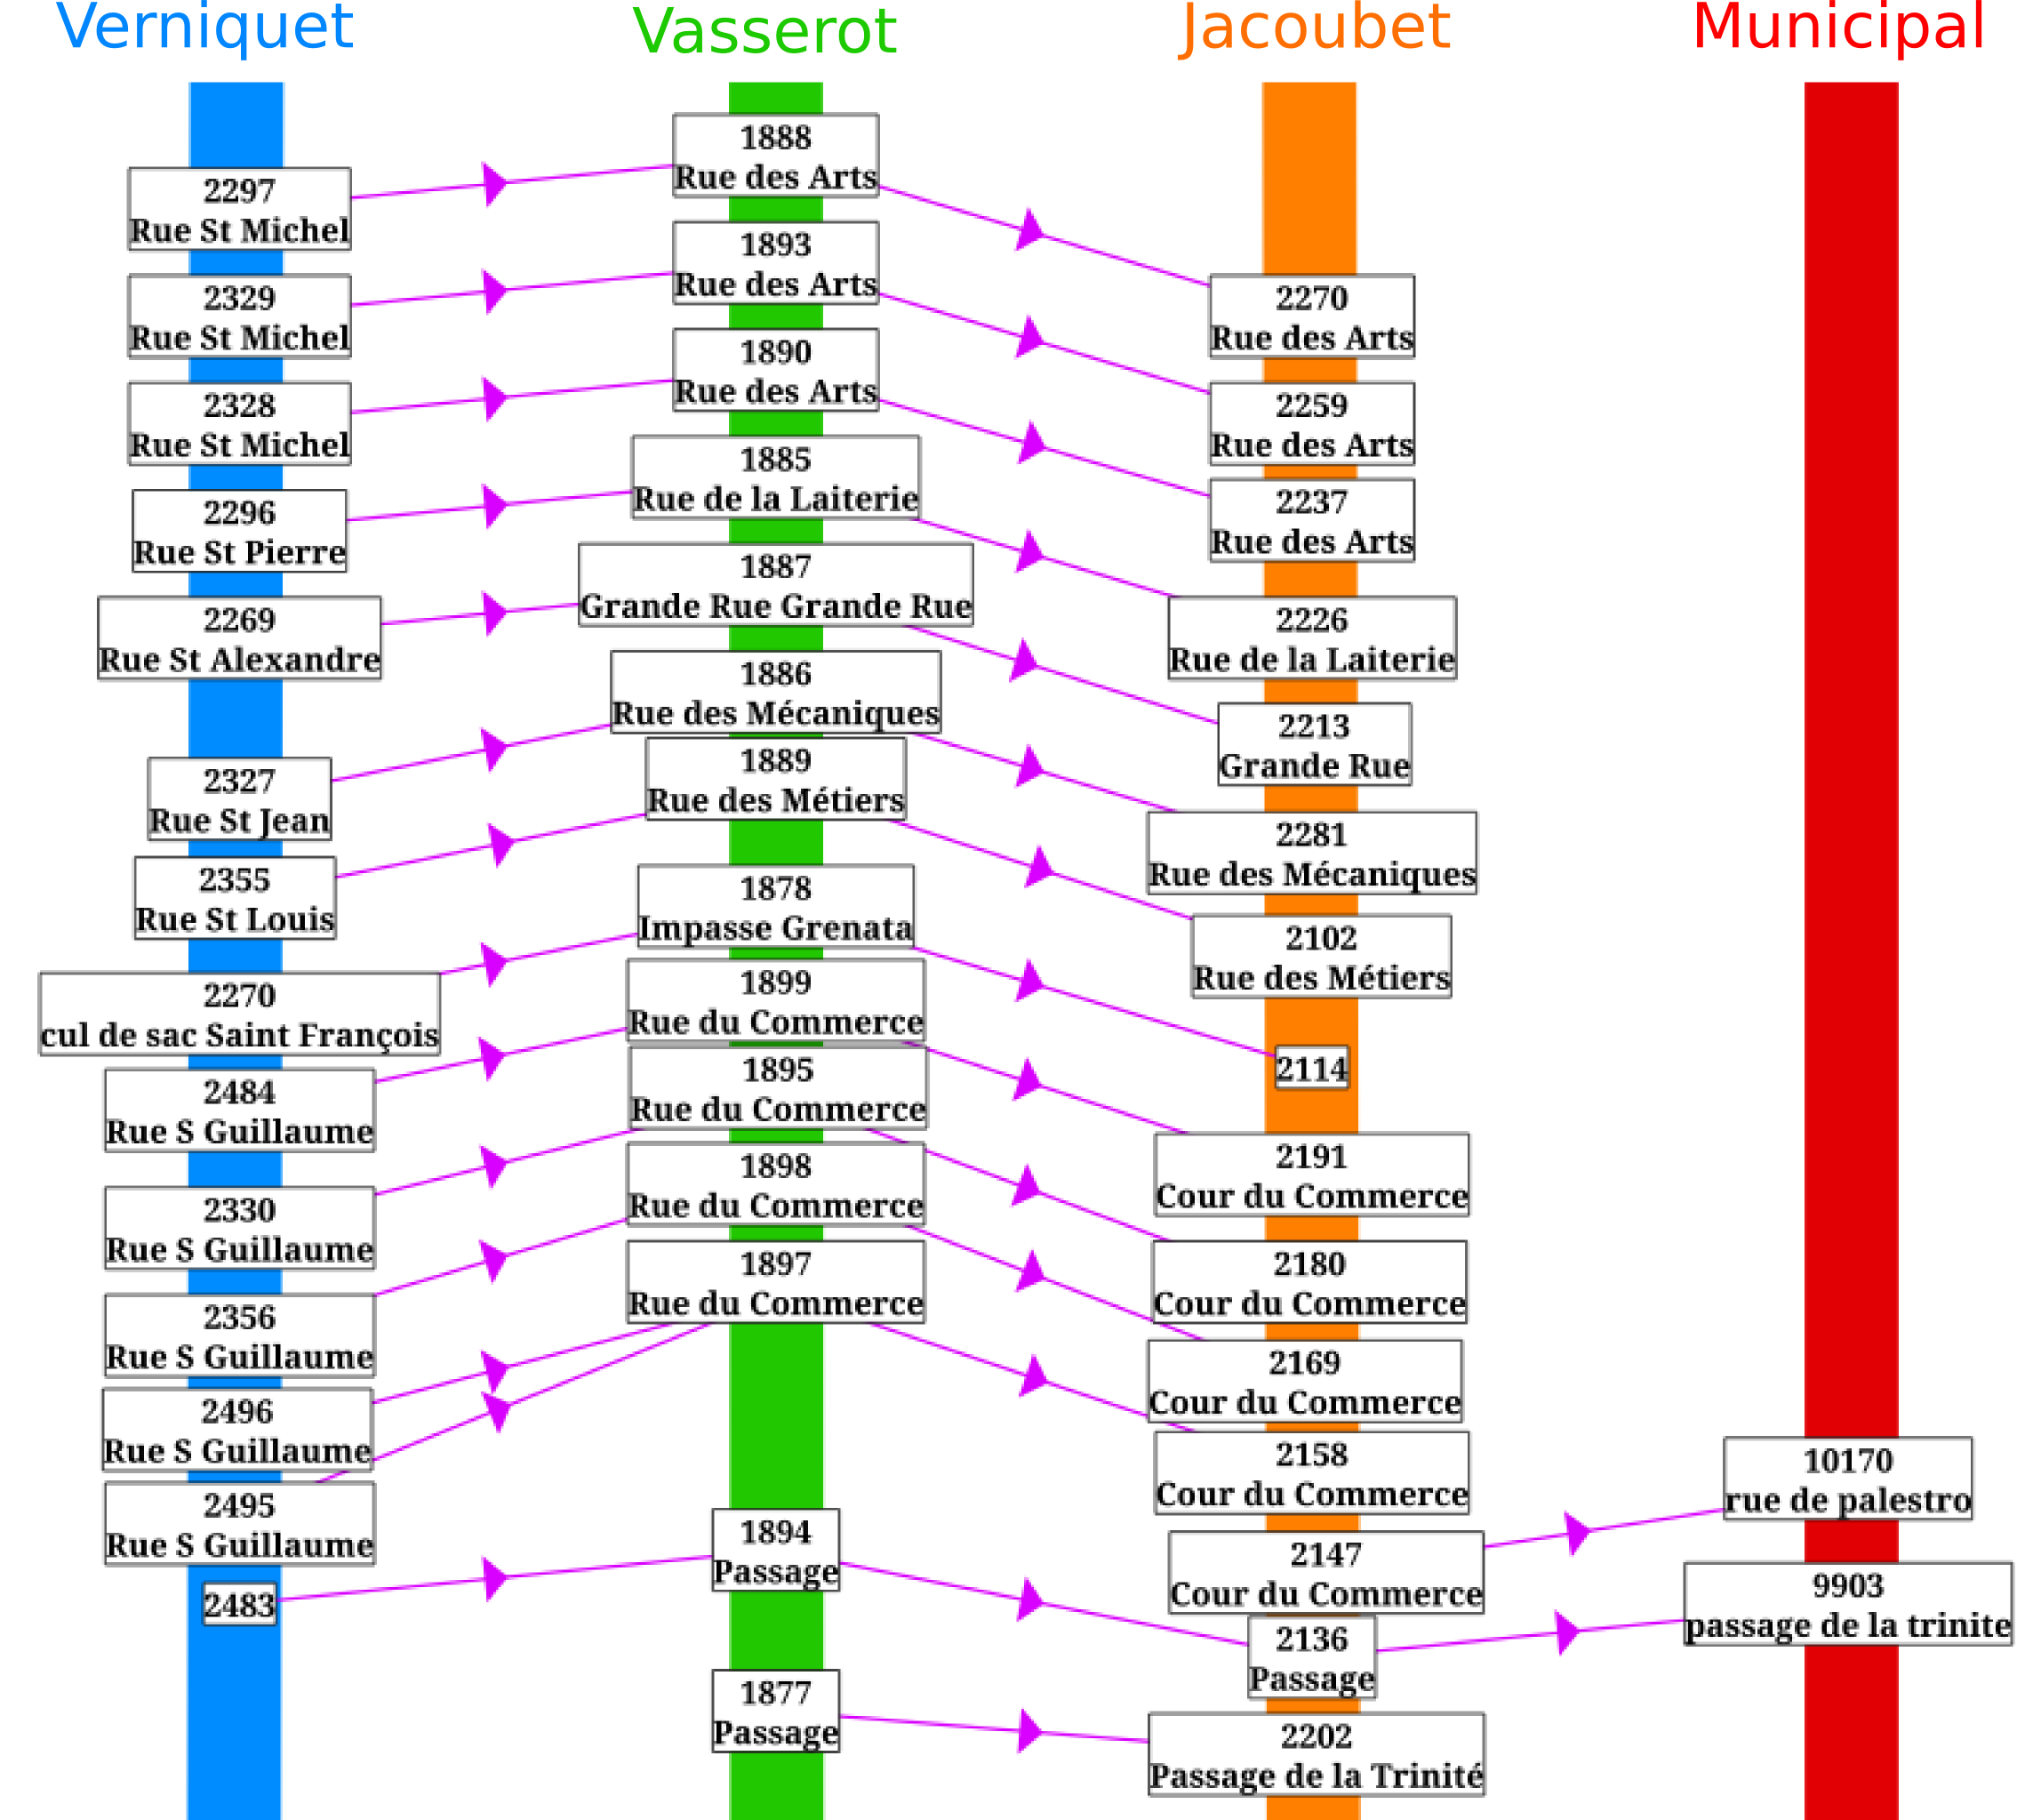
\includegraphics[width=0.8\paperwidth]{./images/illus_graphs/graphe_untagged_greneta.png}
\end{figure}

\begin{figure}
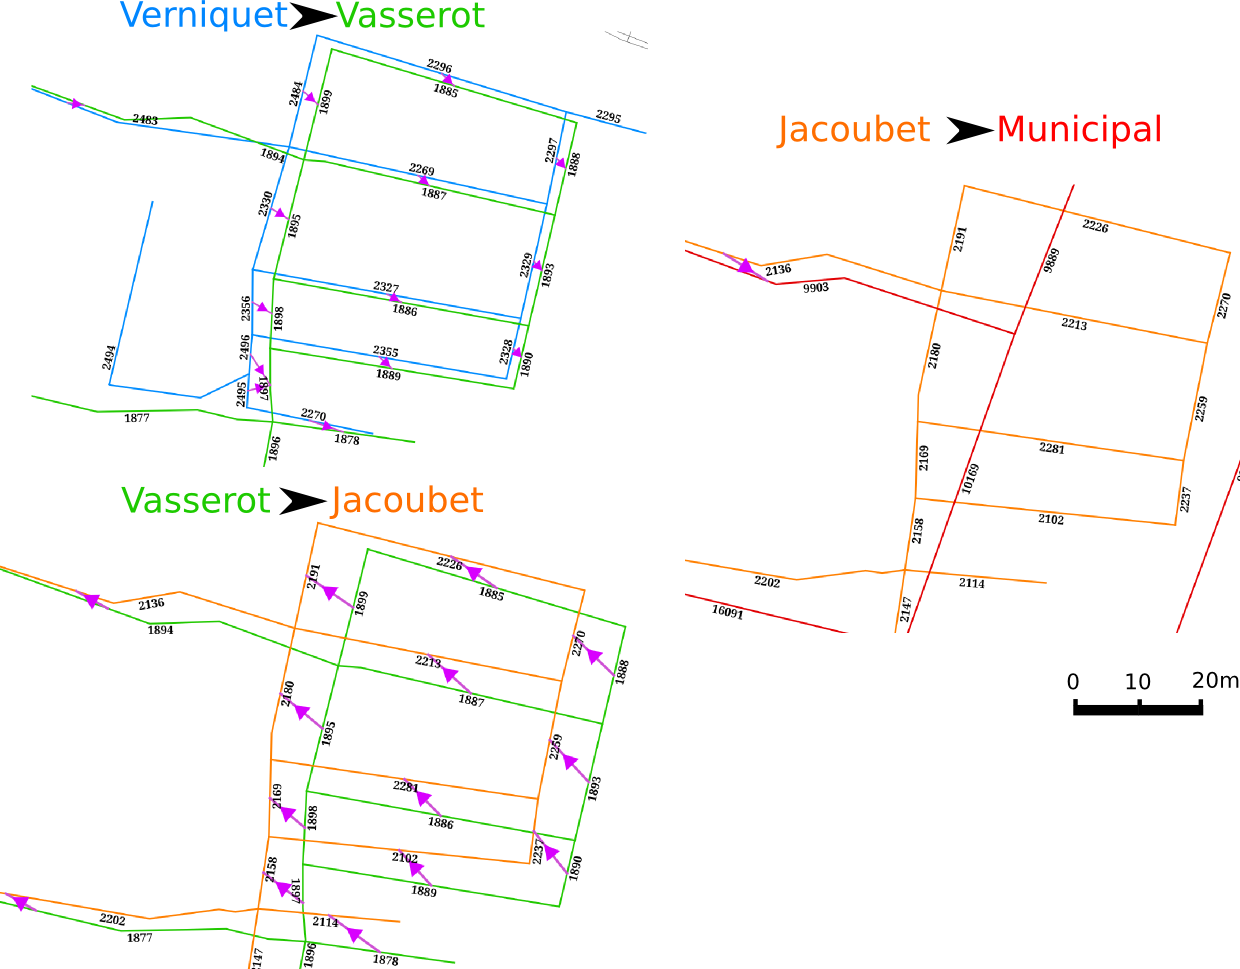
\includegraphics[angle = 90, width=1\textwidth]{./images/illus_graphs/graphe_1_1_greneta.png}
\end{figure}



\begin{figure}
\centering

        \begin{subfigure}[b]{0.5\textheight}
                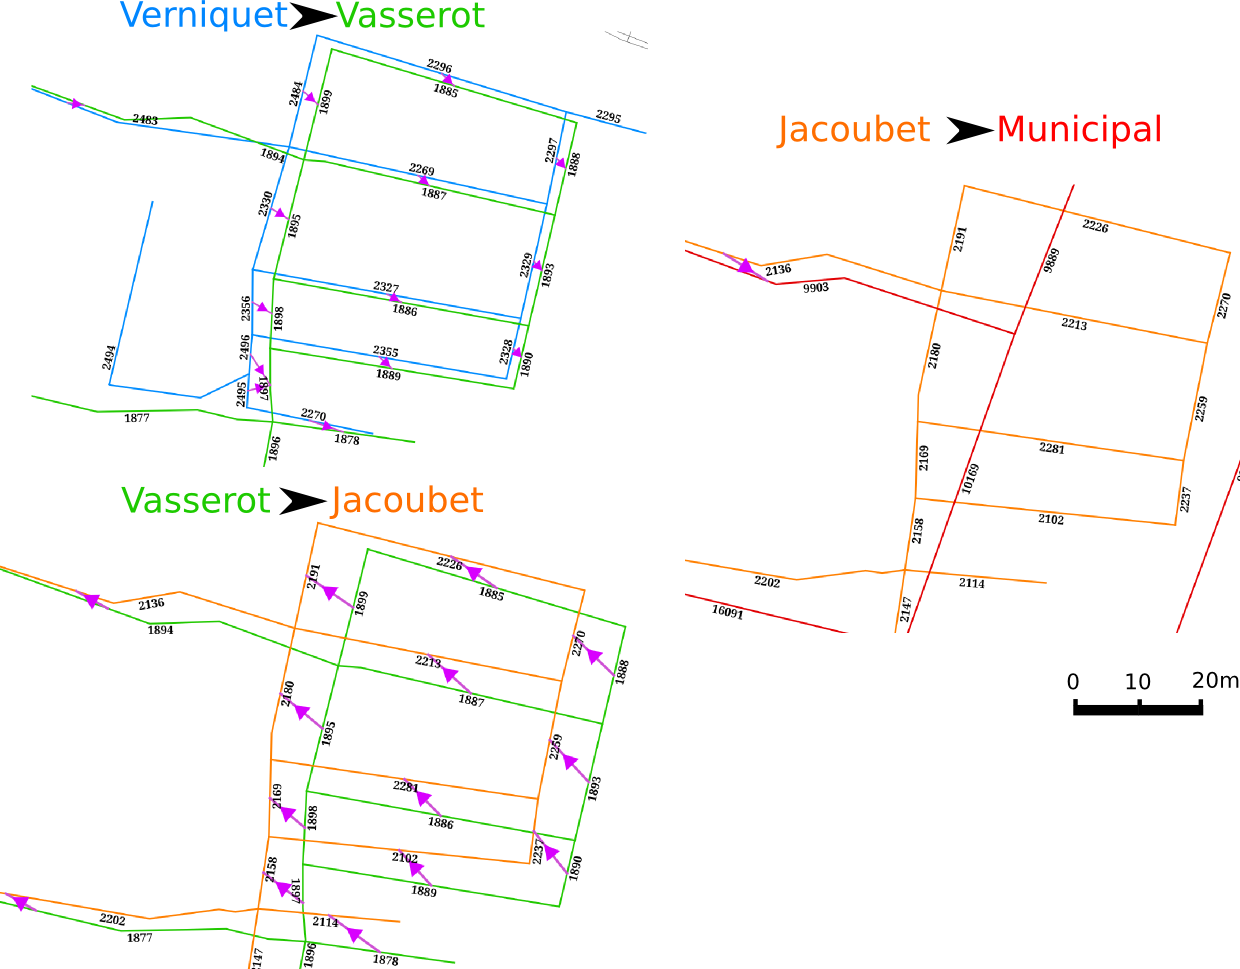
\includegraphics[width=\textwidth]{./images/illus_graphs/graphe_1_1_greneta.png}
				\caption{}
                \label{fig:test}
        \end{subfigure}%v
        \\
                \begin{subfigure}[b]{0.5\textheight}
                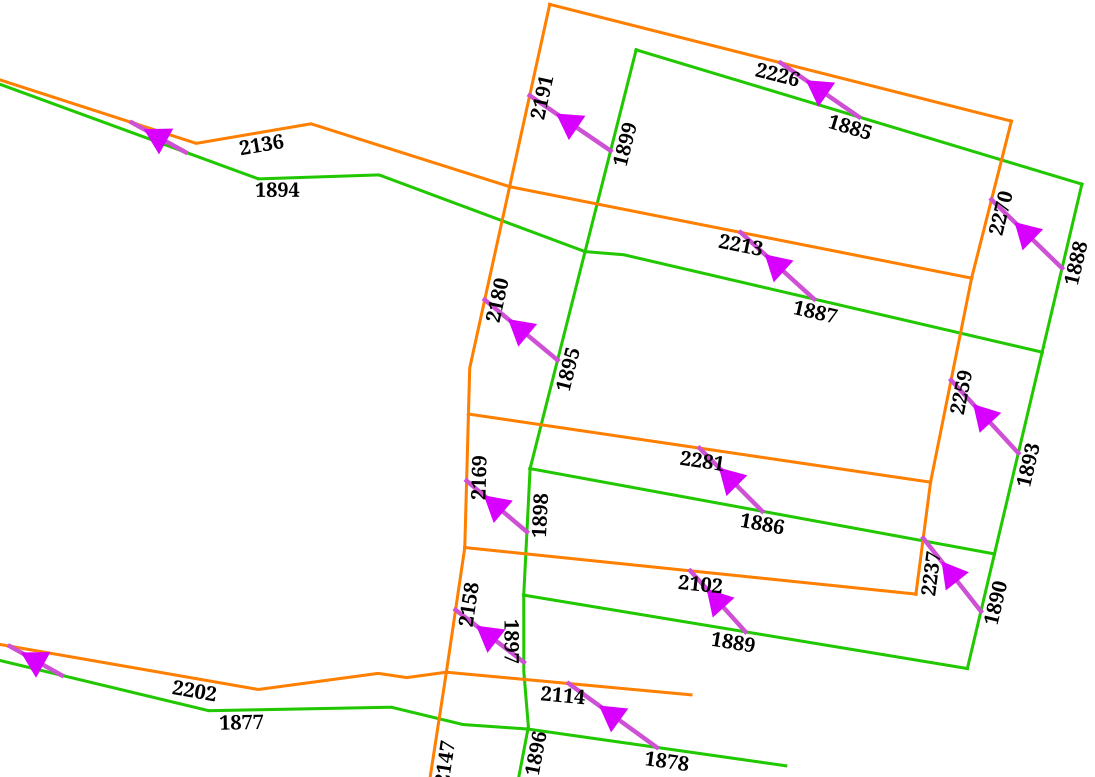
\includegraphics[width=\textwidth]{./images/illus_graphs/graphe_1_1_greneta_2.png}
				\caption{}
                \label{fig:test}
        \end{subfigure}%v
        \end{figure}
\begin{figure}
  \ContinuedFloat 
  \centering

                \begin{subfigure}[b]{0.5\textheight}
                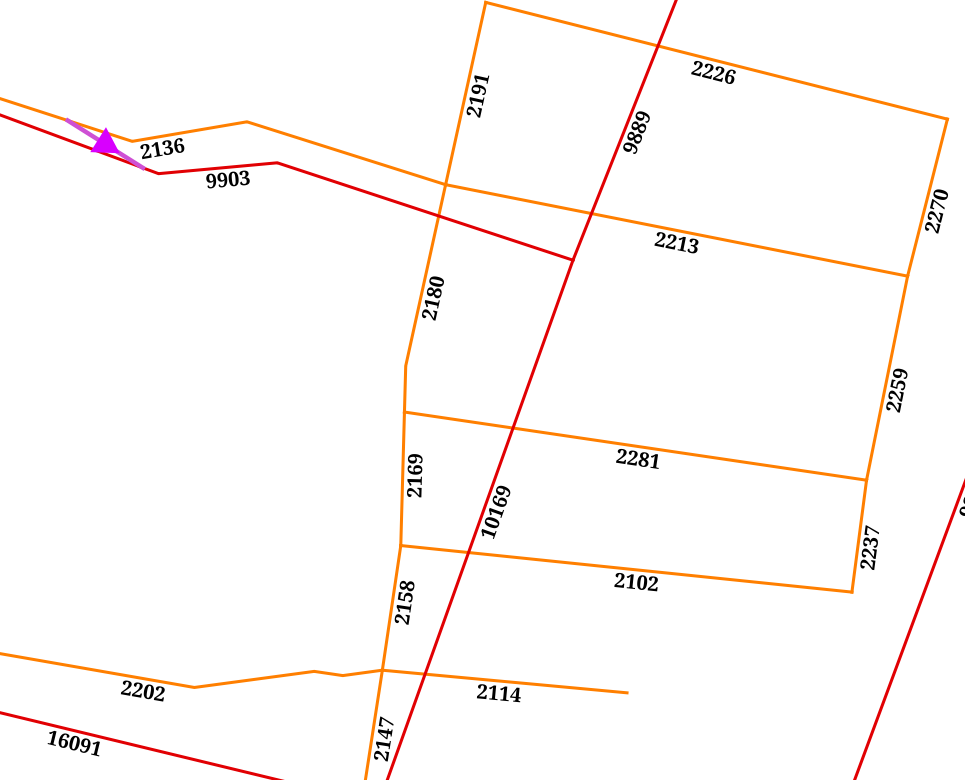
\includegraphics[width=\textwidth]{./images/illus_graphs/graphe_1_1_greneta_3.png}
				\caption{}
                \label{fig:test}
        \end{subfigure}%v
\end{figure}

\subsubsection{Cité}
Stop a 50k iterations. 63.572 secondes (i = 49394)
\\
Strop a 250k iteration : 42.5 minutes (i=188593) 43.6 (i= 192618)

\subsubsection{Saint Martin}
100k iterations.
130 hyperarcs (198 arcs simples)
217.484 seconds
Geometrique : min teps = 1.3,
-1177.886491 


\subsection{Test de la pondération des NM (beta) (TEST DE SENSIBILITE)}
\paragraph{SI beta = 1}
Aucune pondération des NM, l'algo est libre d'en créer. La meilleure solution est trouvée à l'itération.

\begin{figure}
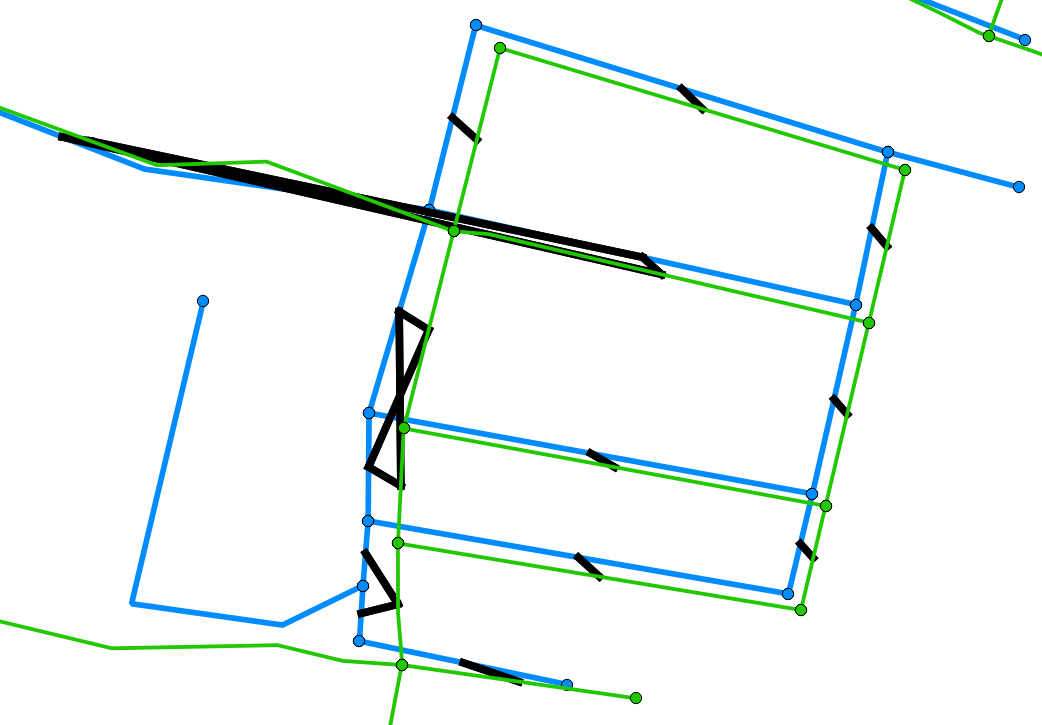
\includegraphics[width=0.8\textwidth]{./images/illus_graphs/greneta_nm_beta1.png}
\end{figure}

\paragraph{SI beta = 0}
Les NMS sont totalement exclus : l'algo n'en créera qu'a haute température
La meilleur solution est trouvée à l'itération~:
\begin{itemize}
\item  r1 =15857
\item  r2 =15857
\item  r3 =15857\\
\item  r4 =15857\\
\item  r5 =15857
\end{itemize}.


-28.145890715773245
-28.145890715773245
-28.14589071577325

Sans le NM du milieu : 
-25.294123
-28.145882 (SANS LE TEMPS)



\end{document}